\section{Some proofs that HLF is not optimal for P3}

This section showcases some situations, where HLF is not optimal. Figure \ref{fig:hlf-001112} an intree, where HLF can choose at some points, and different choices result in different runtimes. 

Figures \ref{fig:hlf-vs-opt-0012346688}, \ref{fig:hlf-vs-opt-0012446788} and \ref{fig:hlf-vs-opt-00123455799} show two examples that prove that HLF is not optimal for three processors.

\begin{figure}[ht]
  \centering
  \begin{subfigure}{.45\linewidth}
    \centering
    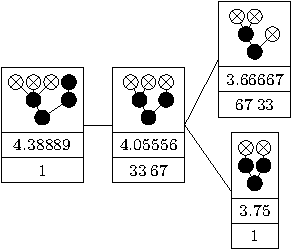
\includegraphics{p3/hlf_not_optimal/001112_hlf_subopt.pdf}
    \caption{Suboptimal HLF run}
  \end{subfigure}
  \begin{subfigure}{.45\linewidth}
    \centering
    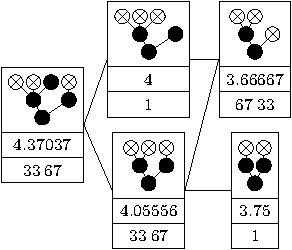
\includegraphics{p3/hlf_not_optimal/001112_hlf_opt.pdf}
    \caption{Optimal HLF run}
  \end{subfigure}
  \caption{HLF on 001112. Different runs of HLF do not necessarily produce the same result.}
  \label{fig:hlf-001112}
\end{figure}

\todo{Explizit auf ambiguity bei HLF hinweisen, und auch dass es klassen von Graphen gibt, die keine HLF-Ambiguity zulassen.}

\begin{figure}[ht]
  \centering
  \begin{subfigure}{.45\linewidth}
    \centering
    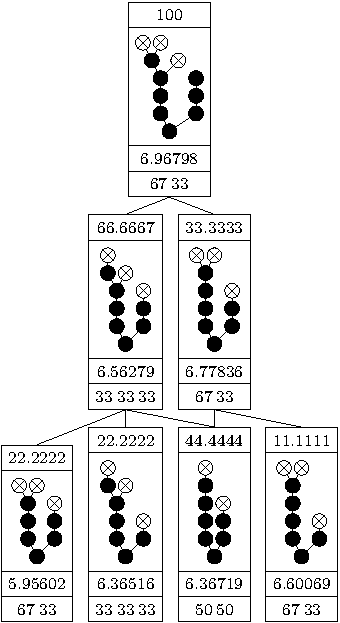
\includegraphics{p3/hlf_not_optimal/0012346688_subopt.pdf}
    \caption{HLF -- suboptimal}
  \end{subfigure}
  \begin{subfigure}{.45\linewidth}
    \centering
    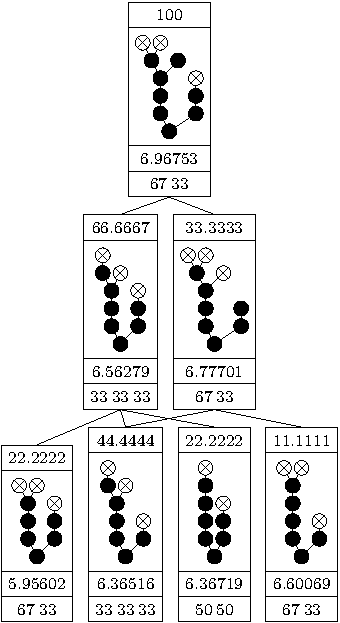
\includegraphics{p3/hlf_not_optimal/0012346688_opt.pdf}
    \caption{Optimal run is non-HLF}
  \end{subfigure}
  \caption{HLF vs. optimal solution for 0012346688}
  \label{fig:hlf-vs-opt-0012346688}
\end{figure}

\begin{figure}[ht]
  \centering
  \begin{subfigure}{.45\linewidth}
    \centering
    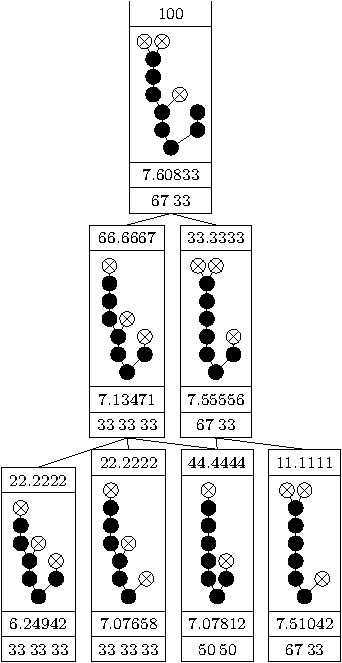
\includegraphics{p3/hlf_not_optimal/0012446788_subopt.pdf}
    \caption{HLF -- suboptimal}
  \end{subfigure}
  \begin{subfigure}{.45\linewidth}
    \centering
    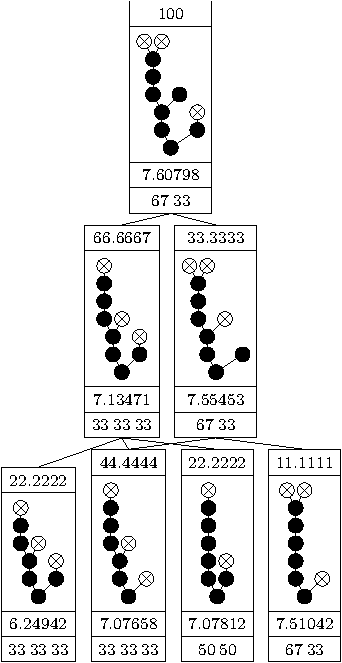
\includegraphics{p3/hlf_not_optimal/0012446788_opt.pdf}
    \caption{Optimal run is non-HLF}
  \end{subfigure}
  \caption{HLF vs. optimal solution for 0012446788 (taken from Ernst Mayr)}
  \label{fig:hlf-vs-opt-0012446788}
\end{figure}

\begin{figure}[ht]
  \centering
  \begin{subfigure}{.45\linewidth}
    \centering
    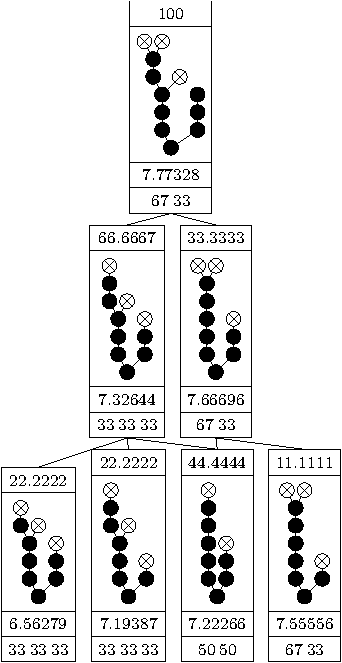
\includegraphics{p3/hlf_not_optimal/00123455799_subopt.pdf}
    \caption{HLF -- suboptimal}
  \end{subfigure}
  \begin{subfigure}{.45\linewidth}
    \centering
    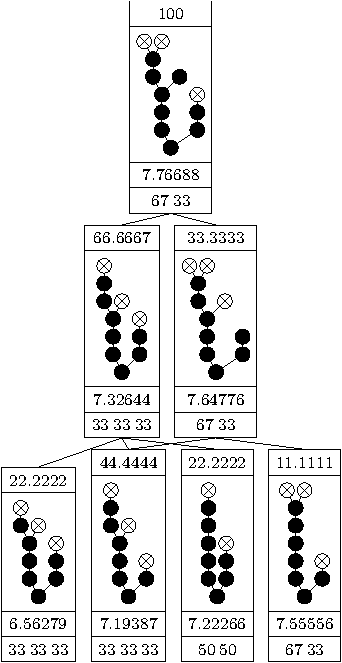
\includegraphics{p3/hlf_not_optimal/00123455799_opt.pdf}
    \caption{Optimal run is non-HLF}
  \end{subfigure}
  \caption{HLF vs. optimal solution for 00123455799 (taken from Chandy/Reynolds)}
  \label{fig:hlf-vs-opt-00123455799}
\end{figure}

%%% Local Variables:
%%% TeX-master: "../thesis.tex"
%%% End: 